\section{Wasserstein距离}
\label{sec:dcomp-wasserstein}

回到章首的两个单点分布$\delta_0$与$\delta_h$。总变差是$1$，Hellinger距离是$1$，KL散度是$+\infty$，这些量都认为两者“完全不同”，无论$h$多小。它们只比较同一位置上的概率，不知道$0$与$h$离得很近。若取值空间有距离，可以换一种问法：把一个分布的概率质量搬成另一个分布的样子，最少要花多大力气？把概率质量想成一堆土，搬一份土的成本是质量乘以搬运距离，$\delta_0$变成$\delta_h$只需把全部质量搬动$h$，成本是$h$，随$h\to0$趋于零。本节把这个想法写成定义。

\subsection{耦合成本}
\label{sec:dcomp-coupling-cost}

搬运方案要说清每一份质量从哪里来、到哪里去。用概率的语言，就是一个二维分布$\pi(\mathrm{d}x,\mathrm{d}y)$：$\pi$在$(x,y)$附近的质量表示从$x$附近搬到$y$附近的土量。从$x$出发的总量必须是$P$在$x$处原有的量，到达$y$的总量必须是$Q$在$y$处需要的量，即$\pi$的两个边缘分别是$P$与$Q$。

\begin{definition}[耦合]
\label{def:dcomp-coupling}
设$\mu,\nu$分别是$\mathcal{X}$与$\mathcal{Y}$上的概率分布。若$\mathcal{X}\times\mathcal{Y}$上的概率分布$\pi$满足
\begin{equation}
 \pi(A\times\mathcal{Y})=\mu(A),\qquad\pi(\mathcal{X}\times B)=\nu(B)
 \label{eq:dcomp-coupling-marginals}
\end{equation}
对一切可测集$A,B$成立，则称$\pi$为$\mu$与$\nu$的一个\term{耦合}（coupling）。全体耦合记作$\Pi(\mu,\nu)$。
\end{definition}

等价地说，耦合是一对定义在同一概率空间上的随机变量$(X,Y)$的联合分布，$X\sim\mu$，$Y\sim\nu$。耦合总是存在，例如乘积分布$\mu\otimes\nu$，它对应让$X$与$Y$独立。耦合只约束边缘，联合分布本身有很大的选择余地。本节按度量空间上测度的习惯，把两个分布记作$\mu,\nu$；需要与前面的量并列比较时仍写$P,Q$。

距离需要底层空间的几何结构。设$(E,d)$是度量空间，并且完备、可分，这样的空间称为\term{Polish空间}（Polish space）。$\mathbb{R}^{d}$、它的闭子集、可数离散集都是Polish空间。完备可分保证了耦合与最优耦合理论中需要的紧性和可测性，度量空间的基本概念可参考\BookChapterRef{chap:metric-spaces}{卷四第2章“度量空间”}。对$1\leq p<\infty$，记$\mathcal{P}_p(E)$为满足
\begin{equation}
 \int_{E}d(x,x_0)^{p}\,\mu(\mathrm{d}x)<\infty
 \label{eq:dcomp-p-moment}
\end{equation}
的概率分布全体，其中$x_0\in E$是任取的基点；由$d(x,x_1)\leq d(x,x_0)+d(x_0,x_1)$，换一个基点不改变有限性。

\begin{definition}[Wasserstein距离]
\label{def:dcomp-wasserstein}
设$(E,d)$是Polish空间，$1\leq p<\infty$，$\mu,\nu\in\mathcal{P}_p(E)$。称
\begin{equation}
 W_p(\mu,\nu)=\Bigl(\inf_{\pi\in\Pi(\mu,\nu)}\int_{E\times E}d(x,y)^{p}\,\pi(\mathrm{d}x,\mathrm{d}y)\Bigr)^{1/p}
 \label{eq:dcomp-wasserstein-def}
\end{equation}
为$\mu$与$\nu$之间的$p$阶\term{Wasserstein距离}（Wasserstein distance）。
\end{definition}

有限矩条件保证下确界有限。用独立耦合，再用$(a+b)^{p}\leq2^{p-1}(a^{p}+b^{p})$与$d(x,y)\leq d(x,x_0)+d(x_0,y)$，
\[
 \begin{aligned}
 &\int d(x,y)^{p}\,(\mu\otimes\nu)(\mathrm{d}x,\mathrm{d}y)\\
 &\qquad\leq2^{p-1}\Bigl(\int d(x,x_0)^{p}\,\mu(\mathrm{d}x)+\int d(x_0,y)^{p}\,\nu(\mathrm{d}y)\Bigr)<\infty .
 \end{aligned}
\]
$W_p$是$\mathcal{P}_p(E)$上的距离。对称与非负直接来自定义；$W_p(\mu,\nu)=0$推出$\mu=\nu$，要用到下确界可以被某个耦合达到；三角不等式要把$\mu$到$\nu$与$\nu$到$\rho$的两个耦合沿公共边缘$\nu$粘合成一个三维分布，用到第~\ref{chap:conditional-distributions}章的正则条件分布。这两步的证明较长，读者可查阅~\scite{math-villani2009transport}。怎样求出最优耦合以及相应的算法由第~\ref{chap:optimal-transport}章研究。

\paragraph{单点分布}
$\delta_x$与$\delta_y$的耦合只有一个：两个边缘都是单点，联合分布只能是$\delta_{(x,y)}$。于是
\[
 W_p(\delta_x,\delta_y)=d(x,y) .
\]
图~\ref{fig:dcomp-point-shift}把它与前面的比较量放在一起：随着平移量$h$变小，$W_p=h$连续地趋于零，总变差与Hellinger距离却一直停在$1$。高斯核MMD介于两者之间：$h$小时它约等于$h$，$h$大时趋于$\sqrt2$，因为核只能“看见”带宽范围内的距离。

\begin{BookInlineFigure}
 \centering
 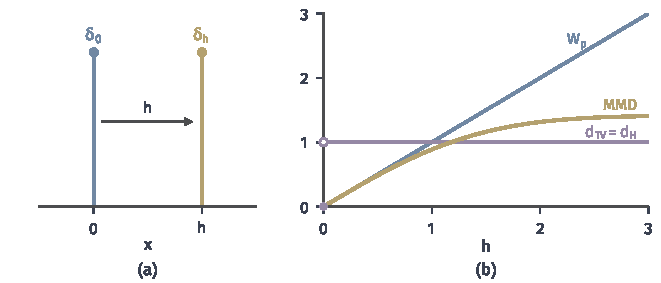
\includegraphics[width=112mm]{figures/07-probability/04-distribution-analysis/matplotlib/dcomp-point-shift/figure.pdf}
 \caption{单点分布的平移。(a)$\delta_0$与$\delta_h$。(b)作为$h$的函数：$W_p=h$（蓝，对所有$p$相同），$d_{\mathrm{TV}}=d_{\mathrm{H}}=1$（紫，$h=0$时为$0$），$\sigma=1$高斯核的$\operatorname{MMD}=\sqrt{2-2\mathrm{e}^{-h^{2}/2}}$（黄）。KL散度对每个$h>0$都是$+\infty$。}
 \label{fig:dcomp-point-shift}
\end{BookInlineFigure}

\paragraph{例表上的搬运}
把例表的三个取值看成实数轴上的位置$0,1,2$，距离取$\lvert x-y\rvert$。耦合是一个$3\times3$的非负矩阵$\bm{\pi}$，行和为$\bm{p}=(0.6,0.3,0.1)$，列和为$\bm{q}=(0.3,0.3,0.4)$，成本是$\sum_{i,j}\bm{\pi}_{i,j}\lvert i-j\rvert^{p}$（下标从$0$起）。图~\ref{fig:dcomp-coupling-plans}给出三个耦合。

\begin{BookInlineFigure}
 \centering
 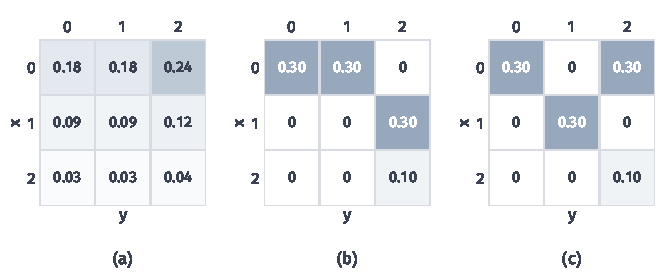
\includegraphics[width=112mm]{figures/07-probability/04-distribution-analysis/matplotlib/dcomp-coupling-plans/figure.pdf}
 \caption{例表的三个耦合，行是$x$（$P$），列是$y$（$Q$），颜色越深质量越大。(a)独立耦合$\bm{p}\bm{q}^{\top}$：$\sum\bm{\pi}_{i,j}\lvert i-j\rvert=0.96$，$\sum\bm{\pi}_{i,j}\lvert i-j\rvert^{2}=1.5$。(b)逐格搬运：两项成本都是$0.6$。(c)跳格搬运：一阶成本$0.6$，二阶成本$1.2$。}
 \label{fig:dcomp-coupling-plans}
\end{BookInlineFigure}

独立耦合让每一份质量都随机地去往目的地，许多质量被不必要地搬远，一阶成本是$0.96$。逐格搬运把点$0$多出的$0.3$搬到点$1$，再把点$1$原有的$0.3$搬到点$2$；跳格搬运直接把$0.3$从$0$搬到$2$，点$1$不动，见图~\ref{fig:dcomp-transport-arrows}。两种方案的一阶成本都是$0.6$。

\begin{BookInlineFigure}
 \centering
 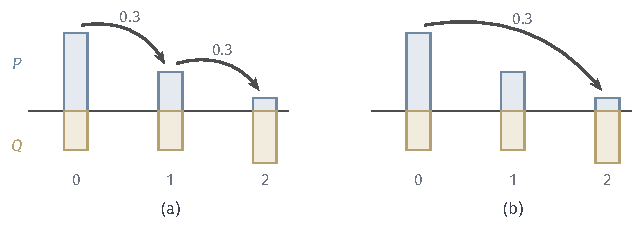
\includegraphics[width=108mm]{figures/07-probability/04-distribution-analysis/tikz/dcomp-transport-arrows/figure.pdf}
 \caption{例表的两种搬运方案，蓝柱向上是$P$，黄柱向下是$Q$，箭头上的数是搬运的质量。(a)逐格搬运：$0\to1$与$1\to2$各$0.3$。(b)跳格搬运：$0\to2$搬$0.3$。}
 \label{fig:dcomp-transport-arrows}
\end{BookInlineFigure}

$0.6$已经是最小值。对任何耦合$(X,Y)$，期望的绝对值不超过绝对值的期望，所以
\[
 \mathbb{E}\lvert X-Y\rvert\geq\lvert\mathbb{E}[X]-\mathbb{E}[Y]\rvert=\lvert0.5-1.1\rvert=0.6 ,
\]
所以$W_1(P,Q)=0.6$，两个方案都最优。二阶成本把两者分开了。记$a=\bm{\pi}_{0,1}$，$b=\bm{\pi}_{0,2}$，$c=\bm{\pi}_{1,2}$。点$0$只能留下$0.3$，所以至少$0.3$离开它，$a+b\geq0.3$；点$2$原有的$0.1$至多满足它的需要$0.4$中的$0.1$，所以$b+c\geq0.3$。成本矩阵中其余元素非负，于是
\[
 \sum_{i,j}\bm{\pi}_{i,j}\lvert i-j\rvert^{2}\geq a+4b+c=(a+b)+(b+c)+2b\geq0.6 ,
\]
等号要求$b=0$，$a=c=0.3$，正是逐格搬运。所以$W_2(P,Q)=\sqrt{0.6}\approx0.7746$。$p=1$时成本按距离线性计，一次跳两格与两次各跳一格花费相同；$p>1$时长距离被加倍惩罚，最优方案倾向于让每份质量只走短路。

这个例子也说明了定义中的“下确界”不能省略。如果$X,Y$已经由某个实验在同一概率空间上给出，它们的联合分布只是$\Pi(P,Q)$中的一个元素，$\mathbb{E}\lvert X-Y\rvert^{p}$通常大于$W_p^{p}$。Wasserstein距离只依赖两个边缘分布，与它们碰巧以怎样的方式一起出现无关。第~\ref{sec:dcomp-wasserstein-convergence}节会再回到这一点。

\paragraph{离散度量下的总变差}
在任意集合上取离散度量$d(x,y)=\mathbf{1}_{\{x\neq y\}}$，搬运成本只问“动没动”，不问距离。这时$W_1$正是总变差：
\begin{equation}
 \inf_{\pi\in\Pi(P,Q)}\pi\bigl(\{(x,y):x\neq y\}\bigr)=d_{\mathrm{TV}}(P,Q) .
 \label{eq:dcomp-maximal-coupling}
\end{equation}
一方面，对任何耦合$(X,Y)$与事件$A$，
\[
 P(A)-Q(A)=\mathbb{P}(X\in A)-\mathbb{P}(Y\in A)\leq\mathbb{P}(X\in A,\,Y\notin A)\leq\mathbb{P}(X\neq Y),
\]
所以左边不小于$d_{\mathrm{TV}}$。另一方面可以构造达到它的耦合。记$\delta=d_{\mathrm{TV}}(P,Q)$，设$0<\delta<1$（$\delta=0$时取$X=Y$，$\delta=1$时任何耦合都满足$\mathbb{P}(X\neq Y)\leq1$）。以概率$1-\delta$令$X=Y$，按密度$\min(p,q)/(1-\delta)$抽取；以概率$\delta$让$X$按密度$(p-q)^{+}/\delta$、$Y$按密度$(q-p)^{+}/\delta$独立抽取。由式~\eqref{eq:dcomp-tv-density}，这些都是概率密度。$X$的密度是$\min(p,q)+(p-q)^{+}=p$，$Y$的密度同理是$q$；第二种情形下$X$落在$\{p>q\}$而$Y$落在$\{q>p\}$，必然不等，所以$\mathbb{P}(X\neq Y)=\delta$。这样的耦合称为\term{最大耦合}（maximal coupling），它让两个变量以尽可能大的概率相等。总变差因此有了一个搬运解释：两个分布重叠的那部分质量原地不动，剩下的$d_{\mathrm{TV}}$那部分必须挪走。

\subsection{一阶距离的函数表示}
\label{sec:dcomp-kr}

例表上，$W_1$的下界来自函数$g(x)=x$的期望差。这不是巧合。若$g$是1-Lipschitz函数，即$\lvert g(x)-g(y)\rvert\leq d(x,y)$，则对任何耦合$(X,Y)$，
\[
 \mathbb{E}_{\mu}[g]-\mathbb{E}_{\nu}[g]=\mathbb{E}\bigl[g(X)-g(Y)\bigr]\leq\mathbb{E}\bigl[d(X,Y)\bigr] .
\]
对耦合取下确界，左边不超过$W_1(\mu,\nu)$。$g$的期望存在，因为$\lvert g(x)\rvert\leq\lvert g(x_0)\rvert+d(x,x_0)$，由一阶矩有限可积。所以每个1-Lipschitz函数都给出$W_1$的一个下界，而每个耦合都给出一个上界。两者在最优处相遇。

\begin{theorem}[Kantorovich--Rubinstein对偶]
\label{thm:dcomp-kantorovich-rubinstein}
设$(E,d)$是Polish空间，$\mu,\nu\in\mathcal{P}_1(E)$。则
\begin{equation}
 W_1(\mu,\nu)=\sup\Bigl\{\mathbb{E}_{\mu}[g]-\mathbb{E}_{\nu}[g]:\ \lvert g(x)-g(y)\rvert\leq d(x,y)\ \text{对一切}\ x,y\Bigr\} .
 \label{eq:dcomp-kr}
\end{equation}
\end{theorem}

上面已经证明了“$\geq$”。下面对两个分布都只有有限个支撑点的情形证明等号，一般情形的证明需要用有限支撑分布逼近并控制紧性，读者可查阅~\scite{math-villani2009transport}。这一结论称为\term{Kantorovich--Rubinstein对偶}（Kantorovich--Rubinstein duality）。

\begin{proof}[有限支撑情形的证明]
设$\mu=\sum_{i=1}^{m}a_i\delta_{x_i}$，$\nu=\sum_{j=1}^{n}b_j\delta_{y_j}$，记$c_{i,j}=d(x_i,y_j)$。两个边缘分别集中在$\{x_i\}$与$\{y_j\}$上，所以耦合集中在这些点对上，由矩阵$\bm{\pi}_{i,j}$描述。$W_1$是线性规划
\[
 \min_{\bm{\pi}\geq\bm{0}}\ \sum_{i,j}c_{i,j}\bm{\pi}_{i,j}\quad\text{s.t.}\quad\sum_{j}\bm{\pi}_{i,j}=a_i,\quad\sum_{i}\bm{\pi}_{i,j}=b_j
\]
的最优值。它的对偶问题是在约束$u_i+v_j\leq c_{i,j}$下最大化$\sum_ia_iu_i+\sum_jb_jv_j$。原问题可行（独立耦合）且目标有下界$0$，由线性规划的强对偶定理，对偶问题有最优解$(\bm{u},\bm{v})$，最优值等于$W_1$，可参考\BookChapterRef{chap:linear-programming}{卷五第2章“线性规划”}。

用对偶解构造一个函数：
\[
 g(z)=\min_{1\leq j\leq n}\bigl(d(z,y_j)-v_j\bigr),\qquad z\in E .
\]
每个$z\mapsto d(z,y_j)-v_j$都是1-Lipschitz函数，有限个1-Lipschitz函数的最小值仍是1-Lipschitz函数。由对偶约束，$u_i\leq c_{i,j}-v_j$对每个$j$成立，所以$g(x_i)\geq u_i$；取$z=y_j$并只看第$j$项，得$g(y_j)\leq-v_j$。于是
\[
 \mathbb{E}_{\mu}[g]-\mathbb{E}_{\nu}[g]=\sum_ia_ig(x_i)-\sum_jb_jg(y_j)\geq\sum_ia_iu_i+\sum_jb_jv_j=W_1(\mu,\nu) .
\]
与已经证明的“$\leq$”合起来，$g$达到了式~\eqref{eq:dcomp-kr}的上确界。
\end{proof}

证明中的$g$由一族“锥形”函数取下包络得到，每个锥以某个$y_j$为顶点、坡度为$1$、整体下移$v_j$。在例表上，$\mu=P$，$\nu=Q$，一个对偶最优解是$\bm{u}=(0,-1,-2)$，$\bm{v}=(0,1,2)$：约束$u_i+v_j=j-i\leq\lvert i-j\rvert$成立，目标值$-0.5+1.1=0.6$。构造出的$g$在$[0,2]$上就是$g(z)=-z$，见图~\ref{fig:dcomp-kr-dual}(b)；它与例表上的下界只差一个符号，$\mathbb{E}_{P}[g]-\mathbb{E}_{Q}[g]=0.6$。图中(a)画出两个分布函数，它们之间的面积也是$0.6$。实数轴上$W_1$与这块面积之间的一般关系属于一维运输问题，在第~\ref{chap:optimal-transport}章讨论。

\begin{BookInlineFigure}
 \centering
 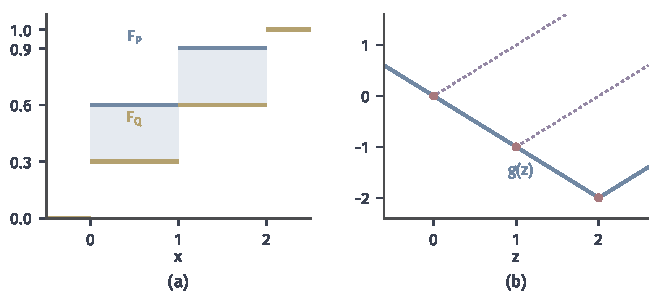
\includegraphics[width=112mm]{figures/07-probability/04-distribution-analysis/matplotlib/dcomp-kr-dual/figure.pdf}
 \caption{例表上的Kantorovich--Rubinstein对偶。(a)分布函数$F_P$（蓝）与$F_Q$（黄），两者之间浅蓝区域的面积为$0.6$。(b)紫色点线是三个锥$\lvert z-y_j\rvert-v_j$，$\bm{v}=(0,1,2)$；蓝线是它们的下包络$g$，红点是$g(x_i)=u_i$。}
 \label{fig:dcomp-kr-dual}
\end{BookInlineFigure}

式~\eqref{eq:dcomp-kr}把$W_1$放进了第~\ref{sec:dcomp-ipm}节的框架：它是由1-Lipschitz函数类生成的积分概率度量。与总变差的式~\eqref{eq:dcomp-tv-dual}对照，总变差的测试函数要求有界、允许跳跃；$W_1$的测试函数要求不能变化太快，但允许无界增长。前者对微小平移敏感，后者对远处的小质量敏感。

\paragraph{高阶距离不是积分概率度量}
$p>1$时，不能把式~\eqref{eq:dcomp-kr}中的$W_1$换成$W_p$，而且任何函数类都不行。原因是积分概率度量沿混合是线性的：对混合分布$\nu_\varepsilon=(1-\varepsilon)\mu+\varepsilon\nu$，每个$g$满足
\[
 \mathbb{E}_{\nu_\varepsilon}[g]-\mathbb{E}_{\mu}[g]=\varepsilon\bigl(\mathbb{E}_{\nu}[g]-\mathbb{E}_{\mu}[g]\bigr),
\]
取上确界得
\[
 d_{\mathcal{G}}(\mu,\nu_\varepsilon)=\varepsilon\,d_{\mathcal{G}}(\mu,\nu) .
\]
取$\mu=\delta_0$与$\nu=\delta_1$，混合分布把$\varepsilon$的质量放在$1$处。最优耦合让$1-\varepsilon$的质量留在原地，把$\varepsilon$的质量搬动距离$1$，所以
\[
 W_p(\mu,\nu_\varepsilon)=\varepsilon^{1/p} .
\]
$p=1$时它是$\varepsilon$，与线性相容；$p=2$时是$\sqrt\varepsilon$，见图~\ref{fig:dcomp-wp-mixture}。若$W_2=d_{\mathcal{G}}$对某个函数类成立，就会有$\sqrt\varepsilon=\varepsilon\cdot1$对一切$\varepsilon\in(0,1)$成立，矛盾。$W_p$对“少量质量走很远”的惩罚是非线性的，这是$p$次方成本带来的。

\begin{BookInlineFigure}
 \centering
 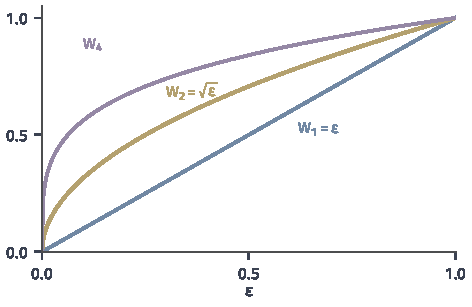
\includegraphics[width=80mm]{figures/07-probability/04-distribution-analysis/matplotlib/dcomp-wp-mixture/figure.pdf}
 \caption{$\delta_0$与$(1-\varepsilon)\delta_0+\varepsilon\delta_1$之间的$W_p=\varepsilon^{1/p}$：$p=1$（蓝），$p=2$（黄），$p=4$（紫）。任何积分概率度量沿这条混合线段都是$\varepsilon$的线性函数，只有$p=1$相容。}
 \label{fig:dcomp-wp-mixture}
\end{BookInlineFigure}
